% !TEX root = ../main.tex
\section{The Population} \label{sec:basicstatistics}
  
  This chapter will be a summary of the basic statistics aggregated from the collected data. Basic statistics is defined as statistics where data are only aggregated and presented as is where no other algorithm or mathematical formulas have been used.

  Background information is the data representing some fundamental aspects on the collected data. This section will go though the data represented in Table \ref{tab:respondentsBasics}, Table \ref{tab:screenlockHabits}, Table \ref{tab:country}, and Figure \ref{fig:ageDistribution} summarizing the basic statistics of the collected data. 

  Table \ref{tab:respondentsBasics} is a overview of the respondents summarizing the frequency of respondents, gender, handedness, their experience with IT and security, and reading/writing orientation. In total 802 respondents completed the whole survey by answering all questions. 11 participants started creating pattern and answering, but stopped before completion. 204 people started creating patterns and stopped before creating all three types of patterns. 81 persons entered the survey and left without leaving any information. 

    %Table: Summary of the background information
    \begin{table}[H]
      \parbox{.45\linewidth}{
        \centering
        \begin{tabular}{ l | l l }
          \hline
          \multicolumn{3}{l}{\bf Respondents} \\ \hline
          Completed survey & 802 \\
          Stoped during survey & 11 \\
          Started creating patterns & 204 \\
          Opened survey and left & 81 \\ \hline
            
          \multicolumn{3}{l}{\bf Gender} \\ \hline
          Male & 529 & 66\% \\
          Female & 278 & 34\% \\ \hline

          \multicolumn{3}{l}{\bf Handedness} \\ \hline
          Left & 97 & 12\% \\
          Right & 690 & 88\% \\ \hline

          \multicolumn{3}{l}{\bf Experience with IT/Security} \\ \hline
          Yes & 470 & 59\% \\
          No & 332 & 41\% \\ \hline

          \multicolumn{2}{l}{\bf Reading/Writing direction} \\ \hline
          Top-to-bottom & 7 & 1\% \\
          Right-to-Left & 8 & 1\% \\
          Left-to-right & 792 & 98\% \\ \hline
        \end{tabular}
        \caption{Summary of the respondents}
        \label{tab:respondentsBasics}
      }
      \hfill
      \parbox{.45\linewidth}{
        \centering
        \begin{tabular}{ l | l l }
          \hline
          \multicolumn{3}{l}{\bf Mobile Operating System} \\ \hline
          Android & 464 & 58.0\% \\
          iOS & 321 & 40.0\% \\
          Windows & 16 & 1.9\% \\
          Blackberry & 1 & 0.1\% \\ \hline
 
          \multicolumn{3}{l}{\bf Used Android Unlock Pattern} \\ \hline
          Yes & 526 & 65\% \\ 
          No & 278 & 35\% \\ \hline

          \multicolumn{3}{l}{\bf Use screenlock} \\ \hline
          Yes & 655 & 82\% \\
          No & 149 & 18\% \\ \hline

          \multicolumn{3}{l}{\bf Screenlock in use} \\ \hline
          Android Pattern Lock & 202 & 31\% \\
          4-digit PIN & 237 & 36\% \\
          Fingerprint & 116 & 18\% \\
          Password & 44 & 7\% \\
          slide-to-unlock & 28 & 4\% \\
          Other & 28 & 4\% \\ \hline
        \end{tabular}
        \caption{Screen lock habits}
        \label{tab:screenlockHabits}
      }
    \end{table}

    Out of the persons entering their gender, 66\% of the participants were male and 34\% were female. Looking at handedness of the participants, 88\% were right-handed and 12\% were left-handed. The percentage of left-handedness in the population is hard to estimate, but it is stated that about 10\% of the population are left-handed \cite{lefthandedness} that seems reasonable with the percentage of left-handed participants from the survey. The reason why the percentage is somehow higher is because the survey was sent to a group of left-handed people that can be the reason for getting 12\% instead of 10\% left-handed participants.
    
    To be able to distinguish between people with experience with IT and Security it was asked about the participants experience in the survey. The network of myself and both supervisors are heavily overrepresented by people in the field of IT and Security. People with this background will might cope with the security related questions in a different way than people without the experience with IT and security. The data shows that the majority, 59\%of the respondents, had a background within IT and Security while 41\% did not. 

    It is hard to reach people outside your own network, especially to reach groups of people with a other cultures. In the dataset it was only 2\% that had an another reading and writing direction, top-to-bottom and right-to-left, than the other participants that read and writhe from left-to-right. Countries operating with a reading and writing direction are often Arabic countries or countries located in Asia. The problem is that many of these countries have during the past years been influenced from western countries. The first problem is to reach people with other reading and writing orientation than myself because all people i know read and write from left to right. I can therefore not make any further statistical analysis comparing people with different reading and writing orientation because the number of participants with that characteristics are too low to get any significant results.

    Table \ref{tab:screenlockHabits} summarized the respondents screenlock habits looking specifically at their experience with the Android Unlock Pattern, their use of screenlock mechanisms, and which screenlock they are currently using. This will provide as a overview of how people cope with security on their smartphones. Because different mobile operating systems provides different security mechanisms, the mobile operating system are also added to the table. It is not a surprise that the majority have answered the survey using either a mobile with a Android or iOs operating system that are the most popular in the the market at this point of time. 

    A total of 65\% of the participants have used the Android Pattern Lock before. The 35\% not familiar with the Android Pattern Lock will probably have their first time using the Android Pattern Lock. There will might be many experienced people with the Android Pattern Lock but it is not given that they are still using it. There are in total 82\% of the participants not using any screenlock and 18\% not using any screenlock. Among the listed screenlocks, the majority are using 4-digit PIN, Android Pattern Lock and fingerprint. The fingerprint are only available at iPhone, while Android Pattern Lock are not allowed on iPhones.

    \clearpage  

    Figure \ref{fig:ageDistribution} shows a distribution of the respondents age. The respondents are divided into 8 intervals: under 20, 20-24, 25-29, 31-34, 35-39, 40-49, 50-59, and over 60. The three last intervals have a lower frequency of participants and have therefore not being divided further into smaller intervals. The distribution have a peak at the interval 20-24. Reasons for the skewed distribution can might be a cause of the network that received the survey. The majority of my own network are students in their twenties and can therefor introduce this skewed distribution. There are still other age intervals represented in the dataset. The higher the age, the lower the frequency of respondents. This can be the same cause as for the peak, but can also be slightly lower respondents over 40 because they do not own a smartphone, nor participate in the networks where the survey were published.

    %Figure: Age distribution
    \begin{figure}[H]
      \centering
      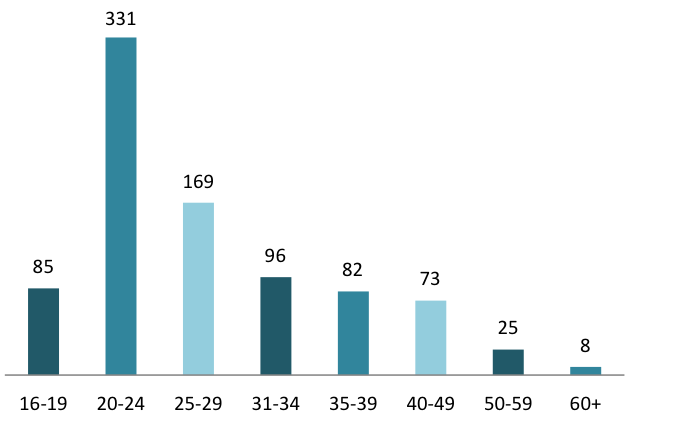
\includegraphics[scale=0.8]{pics/analysis/AgeDist.png}
      \caption{Age distribution}
      \label{fig:ageDistribution}
    \end{figure}

    The survey asked the participants about their country of origin. The data collection ended up with a 39 countries represented in the data set where the majority of the countries was Norway, United States of America as seen in Table \ref{tab:country}.

    This data can not be used to make any analysis on any specific county. During the data collection it was a goal to avoid a homogeneous dataset. The majority of the participants is still from Norway, but is was important to get other countries represented as well to obtain as a more heterogeneous data set. 

		%Table: Country of origin (39 countires)

   {\renewcommand{\arraystretch}{2}%

		\begin{table}[H]
	    \centering
	    \begin{tabular}{ l c | c }
	      \hline
	      \multicolumn{2}{c|}{\bf Country} & {\bf \# Respondents} \\ \hline
	      \raisebox{-.4\height}{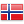
\includegraphics[scale=0.4]{pics/flags/Norway.png}} & Norway & 517 \\ \hline
	      \raisebox{-.4\height}{
\includegraphics[scale=0.4]{pics/flags/USA.png}} & United States of America & 115 \\ \hline
	      \raisebox{-.4\height}{
\includegraphics[scale=0.4]{pics/flags/Germany.png}} & Germany & 33 \\ \hline
	      \raisebox{-.4\height}{
\includegraphics[scale=0.4]{pics/flags/CzechRepublic.png}} & Czech Republic & 31 \\ \hline
	      \raisebox{-.4\height}{
\includegraphics[scale=0.4]{pics/flags/UnitedKingdom.png}} & United Kingdom & 22 \\ \hline
	      \raisebox{-.4\height}{
\includegraphics[scale=0.4]{pics/flags/Russia.png}} & Russia & 13 \\ \hline
	      \raisebox{-.4\height}{
\includegraphics[scale=0.4]{pics/flags/Denmark.png}} & Denmark & 7 \\ \hline
	      \raisebox{-.4\height}{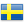
\includegraphics[scale=0.4]{pics/flags/Sweden.png}} & Sweden & 6 \\ \hline
	      \raisebox{-.4\height}{
\includegraphics[scale=0.4]{pics/flags/Switzerland.png}} & Switzerland & 6 \\ \hline
	      \raisebox{-.4\height}{
\includegraphics[scale=0.4]{pics/flags/Australia.png}} & Australia & 5 \\ \hline
	      \raisebox{-.4\height}{
\includegraphics[scale=0.4]{pics/flags/Netherlands.png}} & Netherlands & 4 \\ \hline
	      \raisebox{-.4\height}{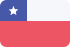
\includegraphics[scale=0.4]{pics/flags/Chile.png}} & Chile & 4 \\ \hline
	      \raisebox{-.4\height}{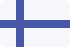
\includegraphics[scale=0.4]{pics/flags/Finland.png}} & Finland & 3 \\ \hline
	      \raisebox{-.4\height}{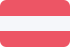
\includegraphics[scale=0.4]{pics/flags/Austria.png}} & Austria & 3 \\ \hline
	      \raisebox{-.4\height}{
\includegraphics[scale=0.4]{pics/flags/Ukraine.png}} & Ukraine & 3 \\ \hline
	      \raisebox{-.4\height}{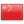
\includegraphics[scale=0.4]{pics/flags/China.png}} & China & 3 \\ \hline
	      \multicolumn{2}{p{8cm}|}{Afghanistan, Mexico, North Korea, Pakistan, Vietnam, Luxembourg, Ireland, Tunisia} & 2 \\ \hline
	      \multicolumn{2}{p{8cm} |}{Italy, Greece, Belgium, Indonesia, Malaysia, Bahrain, Botswana, Argentina, Singapore, japan, Canada, South Korea, Hungary, Turkey, Brazil} & 1 \\ \hline
	    \end{tabular}
	    \caption{Respondents country of origin}
	    \label{tab:country}
	  \end{table}

  {\renewcommand{\arraystretch}{1}%
    


